\documentclass{mathos}

\usepackage{tikz}
\usetikzlibrary{arrows.meta, positioning}

\begin{document}
\renewcommand\bibname{Literatura}


\begin{titlepage}
\begin{center}
    
\includegraphics[keepaspectratio=true,scale=0.4]{MathosLogo.png} \\ \vspace{1mm}
       \textsc{Sveučilište Josipa Jurja Strossmayera u Osijeku} \\
    \vspace{2mm}
    \textsc{Odjel za matematiku}
\end{center}

\begin{center}
    \vspace{4mm}
     {Sveučilišni diplomski studij matematike \\ smjer: Matematika i računarstvo}
\end{center}

\vspace{25mm}
\begin{center}
    {\LARGE{\bf  OWASP Top 10: SQL Injection napadi i zaštita}}

    \vspace{15mm}
    {\large{\sc Seminarski rad}}
\end{center}

\vspace{50mm}

\begin{flushright}
	{\large{\bf Jurica Jurčević}}
\end{flushright}

\vspace*{\fill}
\centering{\normalsize{Osijek, 2026.}}
\end{titlepage}


\tableofcontents
\thispagestyle{empty}


\chapter{Uvod}\label{Uvod}
\pagenumbering{arabic}

\noindent
SQL injection je napad u kojem se ulaz korisnika probije iz podatkovnog dijela upita u njegov naredbeni dio. Aplikacija očekuje ime ili broj, a napadač pošalje komad SQL koda koji baza posluša. Posljedica je čitanje tuđih podataka, zaobilaženje prijave ili, u težim slučajevima, potpuni nadzor nad serverom baze.

Napad je star koliko i web aplikacije s bazama, a i dalje je aktualan. OWASP Top 10 iz 2021.\ godine svrstava ga u kategoriju \emph{A03: Injection}, koja je pala s prvog na treće mjesto, no i dalje pogađa velik dio testiranih aplikacija \cite{owasp2021}. Razlog dugovječnosti je jednostavan. Spajanje niza znakova u tekst upita djeluje prirodno svakom programeru koji uči raditi s bazom, a posljedice tog spajanja nisu očite dok ih netko ne pokaže.

Ovaj rad opisuje kako napad radi, koje vrste postoje i kako se sprječava. Drugo poglavlje objašnjava mehanizam na razini jednog upita. Treće poglavlje razvrstava napade prema tome kako napadač dolazi do rezultata. Četvrto poglavlje sadrži demonstraciju u kontroliranom okruženju, s bazom koja se stvara u radnoj memoriji i nikad ne izlazi iz procesa. Peto poglavlje pokriva obranu, s naglaskom na pripremljene upite jer oni uklanjaju uzrok, a ne samo simptome. Svi primjeri koda i ispisi u radu proizvedeni su pokretanjem priloženih skripti.


\chapter{Kako nastaje SQL injection}\label{mehanizam}

\section{Podatak i naredba u istom nizu znakova}

Baza podataka prima naredbe kao tekst. Kad aplikacija gradi taj tekst lijepljenjem korisničkog ulaza, granica između onoga što je naredba i onoga što je podatak nestaje. Baza vidi samo gotov niz znakova i izvršava ga u cijelosti.

Pogledajmo tipičan upit za prijavu:

\begin{lstlisting}[language=SQL]
SELECT id, uloga FROM korisnici
WHERE korisnicko_ime = 'ana' AND lozinka_hash = '...';
\end{lstlisting}

\noindent
Vrijednost \verb|'ana'| dolazi iz obrasca za prijavu. Ako je aplikacija sastavila upit ovako:

\begin{lstlisting}[language=PHP]
$upit = "... WHERE korisnicko_ime = '" . $ime . "' AND ...";
\end{lstlisting}

\noindent
onda napadač kroz polje \verb|$ime| ne mora poslati ime. Može poslati \verb|admin' -- |. Nakon lijepljenja baza dobiva:

\begin{lstlisting}[language=SQL]
SELECT id, uloga FROM korisnici
WHERE korisnicko_ime = 'admin' -- ' AND lozinka_hash = '...';
\end{lstlisting}

\noindent
Dva znaka \verb|--| u SQL-u započinju komentar do kraja retka. Sve iza njih baza zanemaruje, uključujući provjeru lozinke. Upit sada vraća redak korisnika \verb|admin| bez ijedne lozinke. Apostrof je zatvorio niz znakova koji je programer otvorio, a ostatak ulaza postao je dio naredbe.

\section{Tok podataka}

Slika~\ref{fig:tok} prikazuje put ulaza kroz ranjivu aplikaciju. Ulaz prolazi kroz preglednik i aplikacijski sloj bez provjere, spaja se u upit i stiže u bazu kao gotova naredba.

\begin{figure}[h!]
\centering
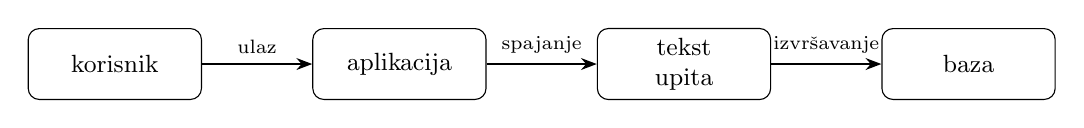
\begin{tikzpicture}[
    node distance=6mm and 14mm,
    box/.style={draw, rounded corners, minimum height=9mm, minimum width=22mm, align=center, font=\small},
    arr/.style={-{Stealth[length=2mm]}, thick}]
\node[box] (u) {korisnik};
\node[box, right=of u] (a) {aplikacija};
\node[box, right=of a] (q) {tekst\\upita};
\node[box, right=of q] (d) {baza};
\draw[arr] (u) -- node[above, font=\scriptsize] {ulaz} (a);
\draw[arr] (a) -- node[above, font=\scriptsize] {spajanje} (q);
\draw[arr] (q) -- node[above, font=\scriptsize] {izvršavanje} (d);
\end{tikzpicture}
\caption{Tok ulaza u ranjivoj aplikaciji. Nigdje se ne razdvaja naredba od podatka.}
\label{fig:tok}
\end{figure}

\noindent
Napad je moguć točno na koraku spajanja. Kad bi taj korak razdvajao tekst upita od vrijednosti, ulaz nikad ne bi mogao promijeniti značenje naredbe. Upravo to rade pripremljeni upiti iz Poglavlja~\ref{obrana}.


\chapter{Vrste napada}\label{vrste}

Napade dijelimo prema tome kako napadač dolazi do informacije. Podjela nije formalna, ali pomaže u razumijevanju obrane jer svaka vrsta traži drukčiji kanal odgovora.

\section{Napadi s izravnim odgovorom}

Kod ovih napada rezultat se vraća u istom odgovoru aplikacije. To je najbrži put jer napadač odmah vidi što je dobio.

\subsection{UNION napad}

Operator \verb|UNION| spaja rezultat dvaju upita u jednu tablicu. Ako napadač zna broj i tip stupaca u izvornom upitu, može dodati vlastiti \verb|SELECT| i pročitati bilo koju tablicu na koju korisnik baze ima pravo. Uvjet je da se broj stupaca poklapa.

\begin{lstlisting}[language=SQL]
' UNION SELECT id, vlasnik, broj FROM kartice --
\end{lstlisting}

\noindent
Ovakav ulaz u polju za pretragu proizvoda vraća sadržaj tablice \verb|kartice| umjesto proizvoda. Demonstracija u Poglavlju~\ref{demo} pokazuje točno ovaj slučaj.

\subsection{Napad kroz poruku o pogrešci}

Ako aplikacija korisniku prikazuje poruke baze o pogreškama, napadač može navesti bazu da vrati podatak unutar same poruke. Primjerice, pretvaranje niza znakova u broj izazove pogrešku koja sadrži taj niz. Ova vrsta danas je rjeđa jer produkcijske aplikacije obično skrivaju detalje pogrešaka, no na testnim i loše postavljenim sustavima i dalje se pojavljuje.

\section{Slijepi napadi}

Kad aplikacija ne vraća ni rezultat upita ni poruke o pogreškama, napadač i dalje može izvlačiti podatke. Postavlja pitanja na koja baza odgovara s da ili ne, i zaključuje po ponašanju aplikacije. Ovo je sporije, jer se svaki bit izvlači zasebno, ali radi.

\subsection{Bulov slijepi napad}

Napadač ubaci uvjet i promatra razliku u odgovoru. Ako se stranica prikaže normalno za \verb|AND 1=1| a drukčije za \verb|AND 1=2|, aplikacija propušta jedan bit informacije po zahtjevu. Nizanjem takvih uvjeta čita se, znak po znak, ime baze, imena tablica i njihov sadržaj.

\subsection{Vremenski slijepi napad}

Kad se odgovor uopće ne mijenja, ostaje vrijeme. Napadač ubaci naredbu koja usporava bazu ako je uvjet istinit, primjerice funkciju koja čeka nekoliko sekundi. Duljina odgovora tada nosi informaciju. Ova varijanta radi čak i kad aplikacija baš ništa ne vraća napadaču, pa je i najsporija.

\section{Napad drugog reda}

Kod napada drugog reda zlonamjerni ulaz se prvo pohrani, naizgled bezopasno, a tek se poslije upotrijebi u nekom drugom upitu. Aplikacija je oprezna pri unosu, ali podatak iz vlastite baze tretira kao pouzdan i lijepi ga u novi upit. Ovo je podmuklo jer provjera na ulazu ne pomaže. Uzrok je isti kao i uvijek, spajanje niza znakova umjesto razdvajanja naredbe od podatka.


\chapter{Demonstracija napada}\label{demo}

\section{Postavljanje}

Demonstracija koristi \verb|sqlite3| iz standardne biblioteke jezika Python i bazu u radnoj memoriji. Ništa se ne sprema na disk i ništa ne izlazi iz procesa. Baza ima tablicu \verb|korisnici| s tri računa i tablicu \verb|kartice| s osjetljivim podacima, kako bi se vidjelo do čega napad može doći.

Skripta uspoređuje dvije inačice funkcije za prijavu. Prva lijepi ulaz u tekst upita, druga koristi pripremljeni upit. Cijeli kod je u prilogu \verb|kod/demo_sqli.py|, a ovdje su ključni dijelovi.

\begin{lstlisting}[language=Python, caption={Ranjiva funkcija za prijavu}, label={lst:ranjiva}]
def prijava_ranjiva(veza, ime, lozinka):
    upit = (
        "SELECT id, korisnicko_ime, uloga FROM korisnici "
        f"WHERE korisnicko_ime = '{ime}' AND lozinka_hash = '{lozinka}'"
    )
    return veza.execute(upit).fetchall()
\end{lstlisting}

\section{Napadi}

Prvi napad zaobilazi provjeru lozinke. Kao korisničko ime pošalje se \verb|admin' -- |, a lozinka je nevažna. Ispis skripte pokazuje upit koji baza stvarno vidi i redak koji je vraćen:

\begin{lstlisting}[basicstyle=\ttfamily\scriptsize]
upit koji baza vidi:
  SELECT id, korisnicko_ime, uloga FROM korisnici
  WHERE korisnicko_ime = 'admin' -- ' AND lozinka_hash = 'bilo sto'
rezultat (1 redaka):
  (3, 'admin', 'administrator')
\end{lstlisting}

\noindent
Prijava je uspjela bez ispravne lozinke. Drugi napad koristi uvjet koji je uvijek istinit, \verb|' OR '1'='1|, u oba polja i vraća sve korisnike odjednom:

\begin{lstlisting}[basicstyle=\ttfamily\scriptsize]
rezultat (3 redaka):
  (1, 'ana', 'korisnik')
  (2, 'marko', 'korisnik')
  (3, 'admin', 'administrator')
\end{lstlisting}

\noindent
Treći napad je UNION. Kao korisničko ime pošalje se sljedeći niz:

\begin{lstlisting}[language=SQL]
' UNION SELECT id, vlasnik, broj FROM kartice --
\end{lstlisting}

\noindent
Upit za korisnike sada vraća sadržaj potpuno druge tablice:

\begin{lstlisting}[basicstyle=\ttfamily\scriptsize]
rezultat (3 redaka):
  (1, 'ana', '4111 1111 1111 1111')
  (2, 'marko', '5500 0000 0000 0004')
  (3, 'admin', '3400 0000 0000 009')
\end{lstlisting}

\noindent
Brojevi kartica nisu ni bili dio prvotnog upita. Napadač ih je dohvatio kroz polje za prijavu.

\section{Ista provjera protiv sigurne inačice}

Sigurna funkcija predaje vrijednosti odvojeno od teksta upita, kroz upitnike:

\begin{lstlisting}[language=Python, caption={Sigurna funkcija za prijavu}, label={lst:sigurna}]
def prijava_sigurna(veza, ime, lozinka):
    upit = (
        "SELECT id, korisnicko_ime, uloga FROM korisnici "
        "WHERE korisnicko_ime = ? AND lozinka_hash = ?"
    )
    return veza.execute(upit, (ime, lozinka)).fetchall()
\end{lstlisting}

\noindent
Isti napadi protiv ove inačice ne rade. Ulaz \verb|admin' -- | tretira se kao doslovno korisničko ime, koje ne postoji, pa prijava vraća prazan skup:

\begin{lstlisting}[basicstyle=\ttfamily\scriptsize]
upit koji baza vidi:
  SELECT ... WHERE korisnicko_ime = ? AND lozinka_hash = ?
  parametri: ("admin' -- ", 'bilo sto')
rezultat (0 redaka):
  prijava odbijena
\end{lstlisting}

\noindent
Razlika nije u provjeri ulaza. Nijedan znak nije uklonjen ni promijenjen. Razlika je u tome što baza sada zna gdje prestaje naredba, a gdje počinje vrijednost.


\chapter{Zaštita}\label{obrana}

\section{Pripremljeni upiti}

Pripremljeni upit (engl.\ \emph{prepared statement}) šalje tekst upita bazi odvojeno od vrijednosti. Baza prvo razumije strukturu naredbe, s praznim mjestima za vrijednosti, a tek onda dobiva podatke. Vrijednost više ne može promijeniti strukturu jer struktura je već određena.

Ovo je jedina mjera koja uklanja uzrok. Sve ostalo su dodatni slojevi. Listing~\ref{lst:sigurna} pokazuje oblik u jeziku Python, a isti pristup postoji u svakom ozbiljnom sučelju prema bazi. U jeziku PHP to je \verb|mysqli::prepare| ili PDO s vezanjem parametara.

Jedno ograničenje treba znati. Kroz parametar se predaju vrijednosti, ne dijelovi sintakse. Ime tablice, ime stupca ili smjer sortiranja ne mogu ići kroz upitnik. Kad ti dijelovi ovise o korisniku, rješenje je bijela lista dopuštenih vrijednosti:

\begin{lstlisting}[language=PHP]
$dozvoljeni = ["asc" => "ASC", "desc" => "DESC"];
$smjer = $dozvoljeni[strtolower($poredak)] ?? "ASC";
\end{lstlisting}

\noindent
Ulaz se ovdje ne ubacuje u upit nego bira jednu od unaprijed poznatih vrijednosti. Nepoznat ulaz padne na sigurnu zadanu vrijednost.

\section{Provjera ulaza}

Provjera ulaza koristi, ali kao dopuna, ne kao zamjena. Ako polje treba sadržavati samo znamenke, odbacivanje svega ostalog smanjuje prostor za napad. Problem je u tome što ispravan ulaz za mnoga polja uključuje apostrof, primjerice prezime \verb|D'Angelo|. Zato provjera ne može biti jedina obrana. Uz pripremljene upite takva imena rade bez ikakvog posebnog rukovanja.

\section{Najmanje ovlasti}

Račun baze kojim se aplikacija spaja treba imati samo ona prava koja mu trebaju. Aplikacija koja samo čita ne treba pravo pisanja ni brisanja. Ako napad ipak uspije, šteta je ograničena onim što taj račun smije. U demonstraciji sigurna inačica koristi račun \verb|webapp_ro| s pravom čitanja, dok ranjiva koristi puni račun.

\section{Slojevi iznad aplikacije}

Web aplikacijski firewall (WAF) pregledava dolazni promet i blokira zahtjeve nalik napadu. Sustav za praćenje bilježi sumnjive upite. Ovi slojevi hvataju napade koje kod propusti i daju vrijeme za reakciju. Ne zamjenjuju ispravan kod jer rade s uzorcima, a napadač uzorke može zaobići. Korisni su kao dodatna crta obrane, ne kao prva.

\begin{table}[hbtp]
\centering
\begin{tabular}{|l|c|l|}\hline
Mjera & Uklanja uzrok & Uloga \\\hline
Pripremljeni upiti & da & osnovna obrana \\\hline
Bijela lista za sintaksu & da & za imena i sortiranje \\\hline
Provjera ulaza & ne & smanjuje prostor napada \\\hline
Najmanje ovlasti & ne & ograničava štetu \\\hline
WAF i praćenje & ne & dodatni sloj \\\hline
\end{tabular}
\caption{Mjere zaštite i njihova uloga.}
\label{tab:mjere}
\end{table}


\chapter{Zaključak}\label{zakljucak}

\noindent
SQL injection ostaje čest jer njegov uzrok djeluje bezazleno. Spajanje ulaza u tekst upita normalan je potez dok netko ne pokaže što se time otvara. Demonstracija u ovom radu prikazala je tri napada na istoj bazi, od zaobilaženja prijave do čitanja tablice koja nije bila dio upita, i sve kroz obično polje obrasca.

Obrana je poznata i nije skupa. Pripremljeni upiti razdvajaju naredbu od podatka i time uklanjaju uzrok, a ne samo pojedini simptom. Provjera ulaza, najmanje ovlasti i slojevi poput WAF-a dodaju sigurnost, ali ne zamjenjuju taj temelj. Aplikacija koja od početka koristi pripremljene upite zatvara cijelu ovu kategoriju napada, i to bez dodatnog troška u odnosu na ranjivu inačicu.


\begin{thebibliography}{30}
\addcontentsline{toc}{chapter}{Literatura}

\bibitem{owasp2021}
{\sc OWASP Foundation}, {\em OWASP Top 10:2021}, dostupno na \verb|https://owasp.org/Top10/|, pristupljeno u kolovozu 2026.

\bibitem{owaspcheat}
{\sc OWASP Foundation}, {\em SQL Injection Prevention Cheat Sheet}, dostupno na \verb|https://cheatsheetseries.owasp.org/|, pristupljeno u kolovozu 2026.

\bibitem{clarke}
{\sc J.~Clarke}, {\em SQL Injection Attacks and Defense}, 2.\ izdanje, Syngress, Waltham, 2012.

\bibitem{cwe89}
{\sc MITRE}, {\em CWE-89: Improper Neutralization of Special Elements used in an SQL Command}, dostupno na \verb|https://cwe.mitre.org/data/definitions/89.html|, pristupljeno u kolovozu 2026.

\bibitem{sqlitedocs}
{\sc SQLite}, {\em Query Language Documentation}, dostupno na \verb|https://sqlite.org/lang.html|, pristupljeno u kolovozu 2026.
\end{thebibliography}


\chapter*{Sažetak}
\markboth{}{SAŽETAK}
\addcontentsline{toc}{chapter}{Sažetak}

SQL injection je napad u kojem korisnički ulaz iz podatkovnog dijela upita prijeđe u njegov naredbeni dio. Rad opisuje mehanizam napada na razini jednog upita, razvrstava napade na one s izravnim odgovorom, slijepe napade i napade drugog reda, te kroz demonstraciju u kontroliranom okruženju pokazuje zaobilaženje prijave i čitanje tuđe tablice. Zaštita se gradi oko pripremljenih upita, koji razdvajaju naredbu od podatka i uklanjaju uzrok napada, uz dodatne slojeve poput provjere ulaza, najmanjih ovlasti i web aplikacijskog firewalla.

\section*{Ključne riječi}

sql injection, sigurnost baza podataka, pripremljeni upiti, owasp, web sigurnost, napad ubacivanjem


\chapter*{Naslov rada na engleskom jeziku}
\markboth{}{SUMMARY}

\section*{Summary}
\addcontentsline{toc}{chapter}{Summary}

SQL injection is an attack in which user input crosses from the data part of a query into its command part. This paper describes the mechanism at the level of a single query, groups attacks into in-band, blind, and second-order types, and demonstrates in a controlled environment how an attacker bypasses login and reads an unrelated table. Defense is built around prepared statements, which separate command from data and remove the root cause, together with supporting layers such as input validation, least privilege, and a web application firewall.

\section*{Keywords}

sql injection, database security, prepared statements, owasp, web security, injection attack


\end{document}
